\documentclass[12pt,a4paper,fleqn, onesside]{report}
%
\usepackage[T1]{fontenc}
\usepackage{amsmath, amssymb, amsthm}
\usepackage[danish,english]{babel}

\usepackage[ansinew]{inputenc}
%\usepackage[utf8]{inputenc} %Der skal anvendes utf8
\usepackage{epsfig}
\usepackage{graphicx}
\usepackage[]{mcode}
\usepackage{lmodern}
\usepackage{float}
\usepackage{setspace}
\usepackage{lscape}
\usepackage{hyperref}
\usepackage{cleveref}
\crefname{equation}{}{equations}
\crefname{figure}{figure}{figures}
\usepackage{tabu}
\usepackage{graphicx}
\usepackage{caption}
\usepackage{multirow}
\usepackage{spverbatim}
\usepackage{dirtytalk}
\usepackage{gensymb}
\usepackage{pdfpages}
\usepackage{mathpazo}
\onehalfspacing

\usepackage[top=25mm, left=30mm, right=30mm,bottom=25mm,headsep=10mm, footskip=12mm]{geometry}
%
\usepackage{fancyhdr}
\pagestyle{fancyplain}
\lhead[\thepage]{}

\begin{document}

% PAGE DE TITRE
\begin{titlepage}
\begin{center}
\vspace{4cm}
\Huge{\sc 30330 Image Analysis with Microcomputer}\\
\vspace{0.8cm}
\large{\sc Project report\\}
\vspace{1.2cm}
%\Huge {\sc Exam Report}\\
%\vspace{2cm}
\normalsize{by}\\
\vspace{1.2cm}
{\sc
\large Katleen Blanchet s150798  \\ 
Titouan Boulmier s150810\\
}
%\o{}
\vspace{2cm}
\begin{center}

\includegraphics[scale=2.2]{dtulogo2.jpg}
\end{center} 
\vspace{3.1cm}
\normalsize{\today}\\
\vspace{1.37cm}
\includegraphics[scale=0.7]{dtulogo.jpg}\\
\vspace{0.2cm}
\normalsize{Technical University of Denmark \\ Department of Electrical Engineering \\
}
\end{center}
\end{titlepage}
%\newpage
\thispagestyle{empty}
\selectlanguage{english}

\pagebreak
\pagenumbering{Roman}
\setcounter{page}{1}
\setcounter{tocdepth}{4}
\setcounter{secnumdepth}{4} 
\def\chaptername{Part}

% SOMMAIRE
\tableofcontents
\newpage
\pagenumbering{arabic}

% Intro
\section*{Introduction}
\addcontentsline{toc}{part}{Introduction au projet}
The research of habitable planet is one of the major concerns of human beings. Indeed, this discovery, in addition to give hope of locating another species, would bring solutions to overpopulation. According to scientists, the main criterion for life is water. Since the properties of celestial bodies are disparate, a habitable zone was defined, considering that water can only exist at a specific range of temperature. If the temperature of the planet is too low, the water will freeze and conversely, it will evaporate if the temperature is too warm. The habitable zone is not fixed; it moves with the evolution of the sun. Mars is thought to have belonged to the zone once, due to its most hospitable climate after Earth. For a matter of fact, NASA's Mars Reconnaissance Orbiter has recently provided a strong evidence of water currently flowing on the Red Planet. It may then be possible to live on Mars and that is the aim of Mars one project: send a colony over there. The terraforming, which would change characteristics of Mars to make it suitable for humans, is also worth considering before colonization. In order to do so, scientists need to learn more about the features of the planet. Orbiters and rovers are already scanning mars surface and soil. Nevertheless, they lack the depth information, only equipped of Two Dimensional (2D) cameras. Their three dimensional (3D) scans have permitted to acquire it and to print a Martian meteorite on Earth in 2014. This information is useful for a better understanding of the rocks properties but that is not enough. Some missing data have delayed the 3D print. It could be interesting to provide to scientists a real time 3D map of a selected rock. It would be easier to study stones but the map could also help the robot to stabilize. With wind and an uneven ground, the rover is liable to move. The pattern recognition of a rock would be more robust by adding a 3D map. Samples could be collected being sure that the robot has taken the right piece. 

Furthermore, the 3D map could have several other applications. The features of the Martian soil acquired by the orbiting satellites are not exhaustive and lack of accuracy. Thus, applied to the area in front of the robot, the 3D map could detect new obstacles and update in real time the available map to distinguish modifications of the ground. It could also permit spacecrafts to determine a flat area to land in real time by analyzing the surface of the planet from space and during the descent. Moreover, the 3D map has other applications in completely different fields. Indeed, this technical can found, as example, in video games with environment recordings for real time augmented reality gaming, in medicine with skin surface measurement or skin roughness measurement, in cosmetic with wrinkle measurement and also in industry with 3D-automated optical inspection, volume measurement or Classification of grinding materials and tools.

However, the 3D mapping is not much used and is still improving. In this context, designing a system capable of carrying out a 3D map of a Martian rock would be profitable for future research. This is the purpose of this project, undertaken during the Image Analysis with Microcomputer course, under the supervision of Alessandro Massaro. Combining image and scene analysis, programming and robotics seems relevant for learning to work as an engineer.

This report is intended to our fellow students. The first part will bring additional knowledge required to understand the next developments. The design of the system is described in the next section, followed by its verification. To end, future work is addressed.

\chapter{Problem formulation and delimitation}
\section{Problem formulation}
\begin{figure}[H]
  \centering
  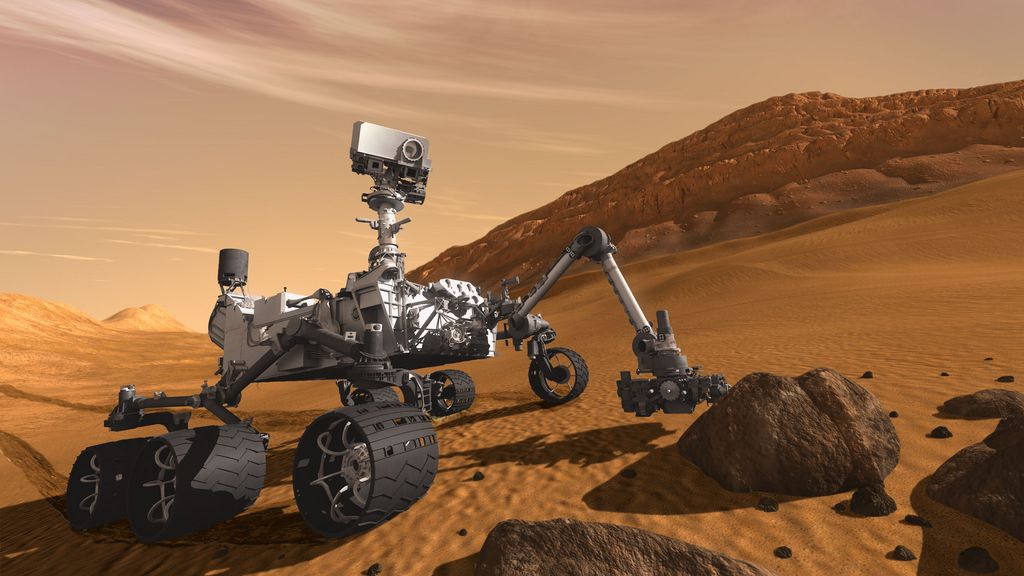
\includegraphics[scale=0.5]{fig/marsRover.jpg}
  \caption{Curiosity Rover with an embedded camera on a arm \cite{nasa}}
  \label{fig:CuriosityRover}
\end{figure}

In this report, we assume that we would like to send a rover on Mars, capable of communicating with Earth. Self-powered by solar panels, it will land at latitude 50� where it could get enough sunlight to recharge its lithium batteries. It is provided with an arm whose hand is replaced with a camera (see figure \ref{fig:CuriosityRover}). The latter will be used by scientists to observe relevant rocks to study. In order to accomplish this mission, once a stone is designed, the camera must be able to keep it in focus, despite the wind, the movement of the robot or any other perturbation. This implies a real time image analysis to be able to rectify the position of the camera. As a robust method is needed to maintain the stone in front of the arm, the correspondence problem is achieved by carrying out a 3D map of the surface. A luminous source should then be added to the rover to be projected on the surface containing the rock and detected by the camera.

This luminous source must be powerful enough to outshine the sunlight during the day, notwithstanding that the energy needed to make it work has to be negligible compared to the amount provided to the rover. Moreover, the characteristics of the camera need to be perfectly adapted to Mars, as once the rover has landed on the red planet, it would be impossible to adjust it. 

Will it be feasible to design such an embedded system, composed of a camera, a luminous source and algorithms, capable of keeping a rock in focus thanks to a 3D map, for an application on Mars soil? 


\section{Problem delimitation}
In order to design the rover's camera which will be used to study rocks and to implement a robust algorithm to carry out a 3D map of the rock's surface, different characteristics of Mars and of the target need to be specified. However, as all of them cannot be taken into account, some simplifications and choices will be assumed.

\paragraph*{Mars delimitation}
~\\
Plenty of missions on Mars have been realized and a great deal of data has already been gathered. Nevertheless, even if some of them will be used to designed our system, others will be simplified or even ignored.
The first simplification concern the atmosphere of Mars. Indeed, even if its composition is now well know, it will be assumed that the dirt on the surface Mars plus the different layers of the atmosphere absorb, or scatter, 10\% of the solar energy. Moreover, the influence on the image acquisition that the dirt between the target and the camera could have will not be taken into account.
The second reduction cover the temperature. Indeed, even if it can reach -143\textdegree C during winter, 27\textdegree C during summer and have around 60\textdegree C variations between daytime and nighttime\cite{wiki:temperature}, we will assume that the CCD sensor works well all the time.

\paragraph*{Target delimitation}
~\\
Regarding the target, that is to say the part of the rock being studied, it is supposed to :
\begin{itemize}
\item be vertical;
\item not exceed 2*2 meters
\item have an area between 0.1 and 1 square meters;
\item have a relief less than  meters.
\end{itemize}

\paragraph*{Camera delimitation}
~\\
Then, regarding the camera which is designed during this study, it is presumed to :
\begin{itemize}
\item be between one and two meters far from the target;
\item be right in front of the target, that is to say that the angle between the normal of the target's surface and the focal axis of the camera is 0\textdegree;
\item be able to capture the image of a target of 2 meters height maximum.
\end{itemize}

The different characteristics of target and the camera are represented figure \ref{fig:schema system}


\begin{figure}[h]
  %\centering
  \centerline{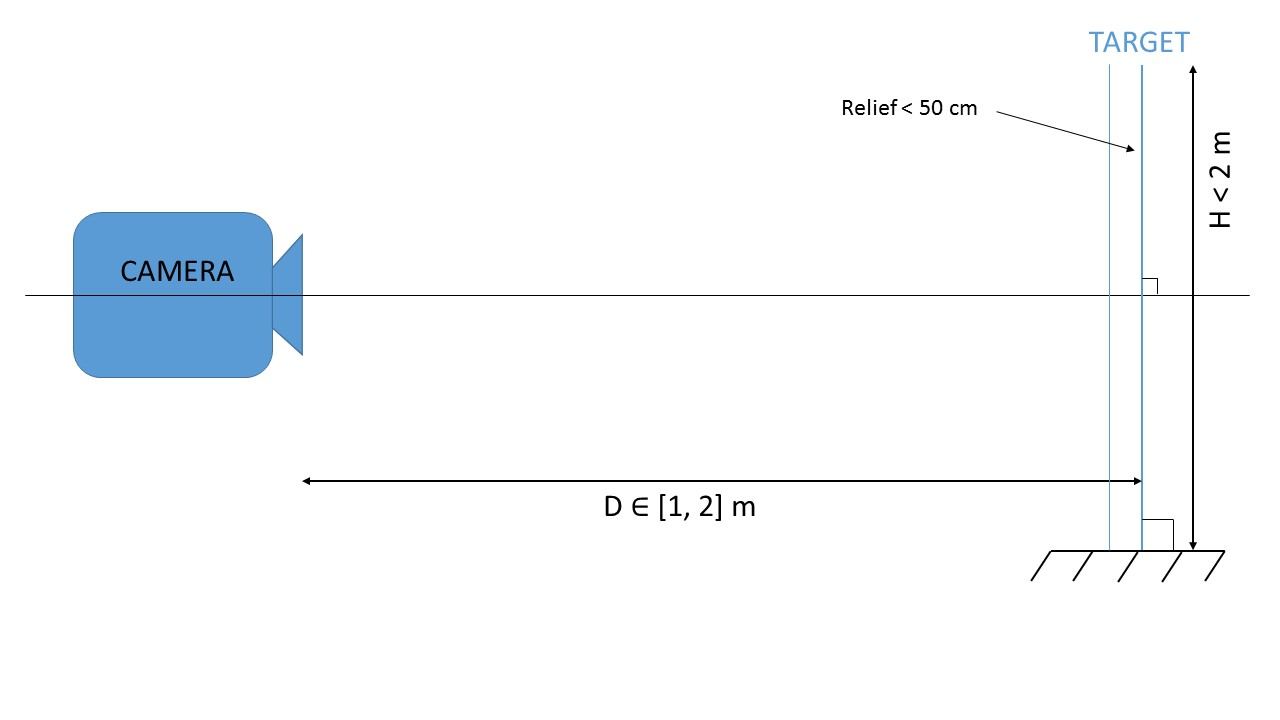
\includegraphics[scale=0.4]{fig/schemaSystem.jpg}}
  \caption{Schema of the scene}
  \label{fig:schema system}
\end{figure}



\chapter{Theory Section}
\section{Mars Features}
Mars, the fourth planet from the Sun (1.3814 to 1.6660 AU) is the second smallest planet of the the Solar System (its radius is 3389.5 km). Known as the ``Red Planet'' because of the amount of iron oxide on its surface, it has an orbital period of 668.6 sols (Mars' solar day), that is to say 687 days, with an average day length of 24h37m.
\subsection{Atmosphere of Mars}
Because of its thin atmosphere, Mars has surface features which present analogies with both Moon, through the impact craters, and Earth, with volcanoes, deserts, polar ice caps. It is mainly composed of carbon dioxide $CO_2$ (96,0 \% $\pm$ 0,7 \%), argon $Ar$ (1,93 \% $\pm$ 0,01 \%) and oxygen
$O_2$ (0,145 \% $\pm$ 0,009 \%). As the gravity of Mars is low, the height of the atmosphere is 11 km, more than one and a half times higher than the Earth's one (7 km). Moreover, due to this low gravity, the wind can disrupt a rover easier than on Earth and a large amount of suspended dust is perpetually present at the surface.

Regarding the dust, of which the particles have a mean diameter of $1,5 \micro m$, is continually injected into the atmosphere by wind or dust devils (a 12 km high one can be seen 12 Figure \ref{fig:poussiere}). Such eddies are far from anecdotal because they bring dust to significant volumes of the atmosphere. Even if the amount of dust is never very massive, it can be lifted by winds slower than 2 $m/s$ and maintained indefinitely by wind of only 0,8 $m/s$.

\begin{figure}[h]
  \centerline{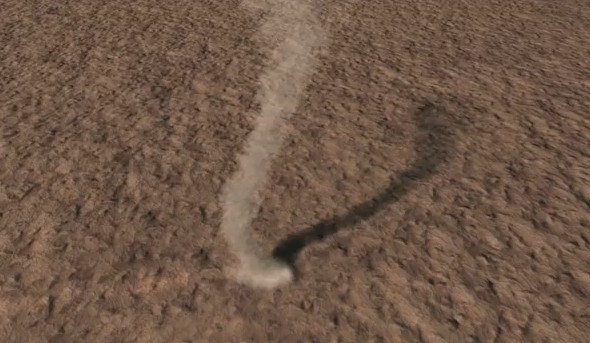
\includegraphics[scale=0.6]{fig/poussiere.jpg}}
  \caption{Dust Devil. Mars Reconnaissance Orbiter, made by HiRISE on Feb. 16, 2012}
  \label{fig:poussiere}
\end{figure}

Moreover, regarding the wind on Mars, in low altitudes, the Hadley circulation\footnote{movement on a planetary level of the layers of gases surrounding the planet} dominate and is almost the same process which, on Earth, generate the Trade winds. In high altitudes, a battery of areas of high and low pressure, named baroclinic pressure waves\footnote{In meteorology a baroclinic atmosphere is one for which the density depends on both the temperature and the pressure}, dominates the weather. The Mars wind lift a large amount of dust and can even trigger huge dust storms which can affect the while atmosphere (see Figure \ref{fig:storm}). Cyclonic storms can also appears on Mars. Indeed, cyclones similar to the ones of Earth tend to create during summer in the northern hemisphere but only in high latitudes.

\begin{figure}[h]
  \centerline{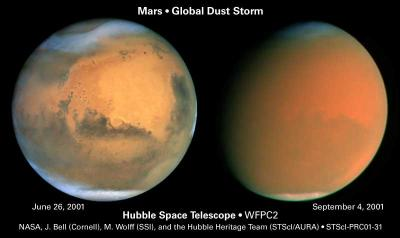
\includegraphics[scale=0.9]{fig/storm.jpg}}
  \caption{Two views of Mars with spatial telescope Hubble before and after the big dust storm in 2001}
  \label{fig:storm}
\end{figure}
\subsection{climate of Mars}
\label{climate}
Because of its distance to the Sun bigger than the one of Earth, Mars receives less solar energy \ref{Irradiance}. Additionally, as its atmosphere is thinner, there is only a negligible greenhouse effect, and hence the average temperature is around -63\textdegree C on the surface of Mars with wide variations between daylight and night. \\
Then, the obliquity of Mars is close to the one of Earth (respectively 25,19\textdegree and 23,44\textdegree) but the eccentricity of Mars is bigger (0,09332 against 0,01671 for Earth) which means that, if Mars has similar seasons to Earth, they have different intensity and duration during the martian year. Thus, the northern hemisphere has seasons less pronounced than the southern hemisphere because its aphelion is at the end of spring and its perihelion at the end of autumn. Thus, there are short and soft winters and long and fresh summers in the northern hemisphere. On the opposite, the southern hemisphere has very pronounced seasons with long and cold winters and short and warmer summers than in the northern hemisphere. That is why there are higher temperature differences in the south.
\subsection{Albedo}
\label{albedo}
Mars surface is covered by sand and volcanic rocks. The first purpose of this project is to allow scientists to examine these rocks through the camera. To achieve it, it is needed to know their characteristics, especially their albedo. As a reminder, the albedo is the fraction of incident light which is reflected from a surface. We can assume that the power reflection of Martian rocks is the same than on Earth. Then, to cover a wild range of rocks, the albedos of a black and of a white stone would be considered. Charcoal, as a dark rock, is a powerful absorber of the sun radiation, with an albedo around 0.05. On the contrary, chalks are poor absorbers and their albedo reach 0.45 according to \cite{albedo}. In the following parts of the report, it will be taken for granted that Martian rocks have an albedo between 5 and 45\%.
\section{Artificial Light Source}
In order to carry out a 3D mapping of the target, the system needs a light source to project points which will be used by the 3D mapping algorithm. In this section, the source of light will be designed.

\subsubsection{Design of the Light Source}
~\\
First of all, the green has been chosen as color of the light source. Indeed, in order to detect easily the points projected on the target, a distinctive color should be used. As we can see figure \ref{fig:QeCCD}, the CCD selected for the camera has the best quantum efficiency for a wavelength around 510 $nm$, which means that the green is the color that is the best recorded by the camera. Secondly, as the surface on Mars is mainly orange, red and brown, this color should stand out.


\begin{figure}[h]
  %\centering
  \centerline{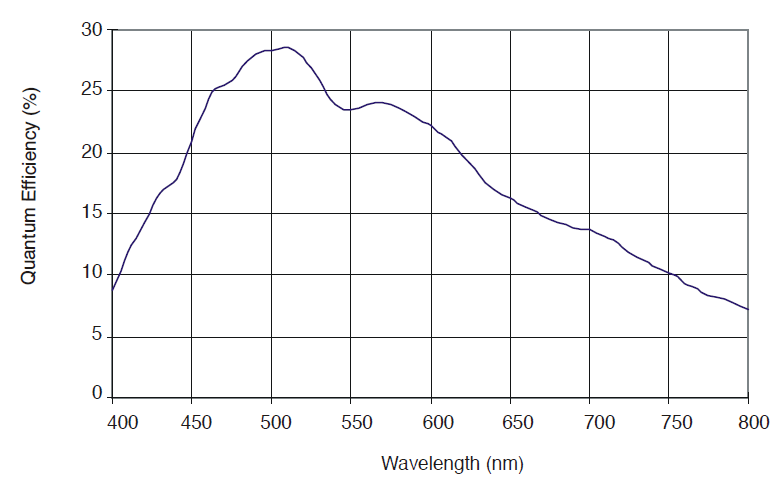
\includegraphics[scale=0.4]{fig/QeCCD.png}}
  \caption{Quantum efficiency versus wavelength of the CCD}
  \label{fig:QeCCD}
\end{figure}

Then, as only 300 $mW$ are available to aliment the light source and a lot of lightning energy is needed to outshine the sunlight, a LED has been chosen. Indeed, LEDs have great energy performances. The properties of the chosen LED can be seen in Annex \ref{LEDdatasheet}. Note that the use of a laser have been studied, but the energy cost would have been too expensive. Moreover, even if we cannot obtained a coherent light, as a laser do, with a LED, it is still feasible to obtain a monochromatic and directional light. Thus, we will assume that the LED can bring enough light (proof in part on Signal Noise Ratio\ref{light Power}).\
Then, as the 3D mapping algorithm needs a grid of points, the LED cannot be used in its present condition. Moreover, lot of light would be lost without an optic system. Thus, a system has been designed to concentrate the luminous beams of the LED and to transform the continuous light into a grid of point. The system uses a lens and a grid (Figure \ref{fig:LEDsystem}). 

\begin{figure}[h]
  %\centering
  \centerline{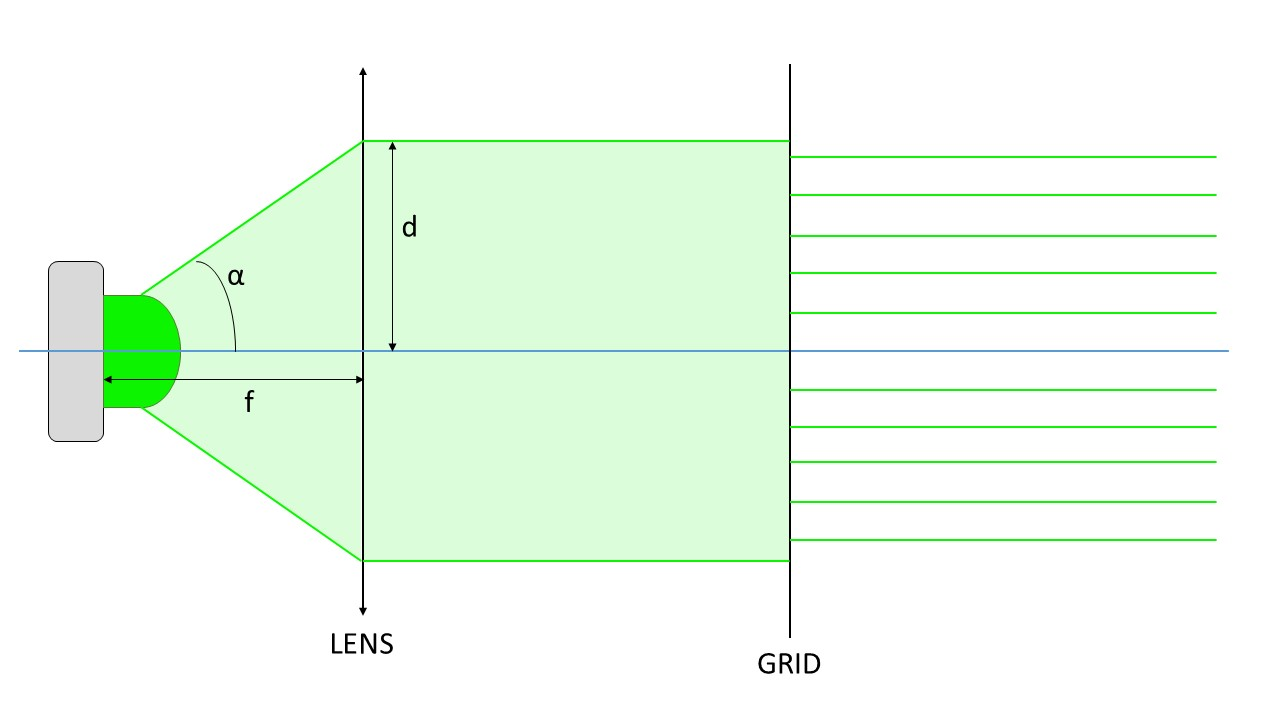
\includegraphics[scale=0.4]{fig/LEDsystem.jpg}}
  \caption{schema of the LED system}
  \label{fig:LEDsystem}
\end{figure}

As the LED has a diffusion angle of 30\textdegree (Annex \ref{LEDdatasheet}), the lens needs to be close enough to collect all the light beams of the LED to avoid losses of energy. In order to capture as much light as possible, the diameter of the lens should follow \eqref{eq:lenseLED}.

\begin{equation}
\label{eq:lenseLED}
d = f \tan \alpha
\end{equation}
with 
\begin{align*}
\alpha & = \frac{30}{2} = 15\mbox{\textdegree, the half of the diffusion angle.}\\
f & \mbox{, the focal length of the lens}
\end{align*}

Moreover, it should be pointed that there is a loss of energy because of the lens and the grid. We will assume that the energy loss coefficient of the lens $LFLLed$ (Loss Factor Lens Led) is 0.5 and the one of the grid $LFGLed$ (Loss Factor Grid Led) is 0.3.

\subsubsection{Validation of the Light Source}
\label{light Power}
~\\
In order to verify weather our light source has enough power or not to outshine the sunlight, the Signal/Noise ratio (SNR) has to be calculated (see part Signal/Noise ratio \ref{thirdcase}). Knowing that 100 is a really great SNR, as the SNR of images recorded with this system is $[32, 348]$, it can be concluded that the LED can be chosen as light source. Indeed, even if 32 is a low ratio, it is only when all the different poor conditions happen in the same time and it does not happen frequently. Moreover, 100 to 347are really high ratios that permit to have the 3D algorithm working well. Thus, the design of the light source is validated.






\chapter{Development}
\section{Scene Analysis}
In order to design the camera and find its characteristics, a scene analysis have to be carried out. Our study is based on the MER (Mars Exploration Rover) cameras properties \cite{merengineeringcameras}.
To begin with, we choose an image sensor. 

\subsubsection{CCD}
\label{fig:CCD}
The Charge Coupled Device (CCD) is commonly more sensitive to light than its counterpart, the CMOS (Complementary Metal Oxide Semiconductor). Moreover, in the near infrared CCD appears to have a better response. Since Mars has a reddish color, it seems more accurate to select the CCD detector.

As scientists will need to discern the details of rocks, the resolution should be around the megapixel. Taking into account the cost, which will increase with the resolution, and the time of computation for an image with too many pixels, 1024 x 1024 seems to be an acceptable compromise.

Finally, the last element to consider is the pixel size. A trade-off have to be found between having a higher resolution (smaller pixels) and more sensitivity (larger pixels). All the camera of the MER mission were conceived with a pixel size of 12 x 12 $\mu m^2$ for a resolution of 1024 x 1024. It was decided to comply with that value.

For the next parts of this report, we will use the data sheet of the FTT1010M CCD image sensor (see Appendix \ref{CCDdatasheet}) as a basis for our calculations which will require CCD details.

\subsubsection{Field of View}
According to the book \cite{book}, the Field of View (FoV) \say{is the angle of the cone of directions encompassed by the scene that is being images}. This solid angle is needed to compute the focal length the camera should have.

\begin{figure}[h]
  \centering
  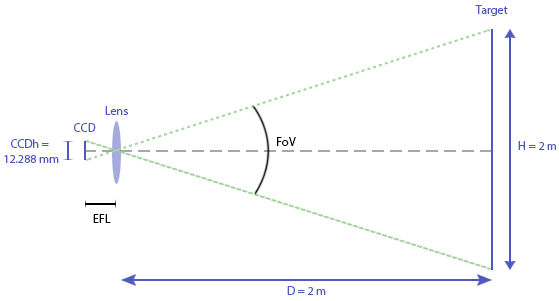
\includegraphics[scale=0.7]{fig/FOV.png}
  \caption{Field of View and Effective Focal Length}
  \label{fig:FOV}
\end{figure}

A simple relationship between the distance lens-target, the size of the target and the FoV can be deduced from the detailed diagram \ref{fig:FOV}: 
\begin{equation*}
tan( \frac{FoV}{2}) = \frac{1}{2} \times \frac{H}{D}
\end{equation*}
We derive and get
\begin{equation*}
 \frac{FoV}{2} = atan(\frac{1}{2} \times \frac{H}{D})
\end{equation*}

Numerically, with our problem delimitation, the Field of View is equal to $26.6\degree \times 26.6\degree$. 

\subsubsection{Focal Length}
\label{focalLength}
Thanks to the previous diagram, the Effective Focal Length (EFL) can also be determined: 
\begin{equation*}
EFL = \frac{1}{2} \times \frac{CCDh}{tan(\frac{FoV}{2})} = 12.29 \ mm
\end{equation*}
where $CCDh$ is the image section of the CCD according to the data sheet.\\

In order to get the real focal length, we choose $rf = 1 \ m$ for the distance of focus of the camera. 
\begin{equation*}
f = \frac{1}{\frac{1}{rf}+\frac{1}{EFL}} = 12.14 \ mm
\end{equation*}

\subsubsection{Aperture}
\label{aperture}
To determine the diameter of the aperture, several criteria have to be accounted for. If the diameter is too small, the sharpness of the image will decrease due to the diffraction effect. In fact, at large aperture, the diffracted light is negligible compared to the total amount of light entering the system. On the other hand, we should also consider the Depth of Field (FoV). We need to insure that it is big enough to allow us to see the whole target on the image. The relationship between the DoF and the diameter is inversely proportional. That means that if we increase the diameter, we will lessen it. The Diameter of Confusion (DoC), linked to the DoF is also a factor to take into consideration for the choice of the diameter. According to Wikipedia \cite{wiki:coc} It corresponds to \say{an optical spot caused by a cone of light rays from a lens not coming to a perfect focus when imaging a point source}. The smaller the DoC is, which corresponds to a better focus, the bigger is the DoF, and also the smaller is the diameter.

As the behaviour of the depth of field and of the diameter of confusion runs counter to the diffraction one, a trade-off has to be found. 

These formula are used to calculate the diameter of confusion and the diffraction spot:
\begin{equation*}
DoC = Dsr \cdot \frac{|r-rf|}{r} \cdot \frac{f}{rf - f}
\end{equation*}
where $Dsr$ is the diameter of the aperture
\begin{equation*}
DiffractionSpot = 2 \cdot EFL \cdot tan(1.22 \cdot \frac{lambda}{Dsr})
\end{equation*}
where $lambda$ is a wavelength of the sunlight\\

In the delimitations, it is assumed that the wavelengths of the sunlight belong to [400 800] nm. To settle on a diameter, the diameter of confusion and the diffraction spot were computed for diameters varying from 1 mm to 5 mm and wavelengths from 400 nm to 800 nm. The results are shown graphically in figure \ref{fig:DoCDifspot}. As the diameter of confusion cannot be bigger than the height of a pixel, the line corresponding to 12 $\mu m$ was also added to the graphic. In order to have the best trade-off, that is to say all the curves under 12 $\mu m$, we have chosen a effective lens entrance aperture $Dsr$ equal to $1.9 \ mm$, corresponding to $DoC = 0.0117 \ mm$. 

\begin{figure}[H]
  \centering
  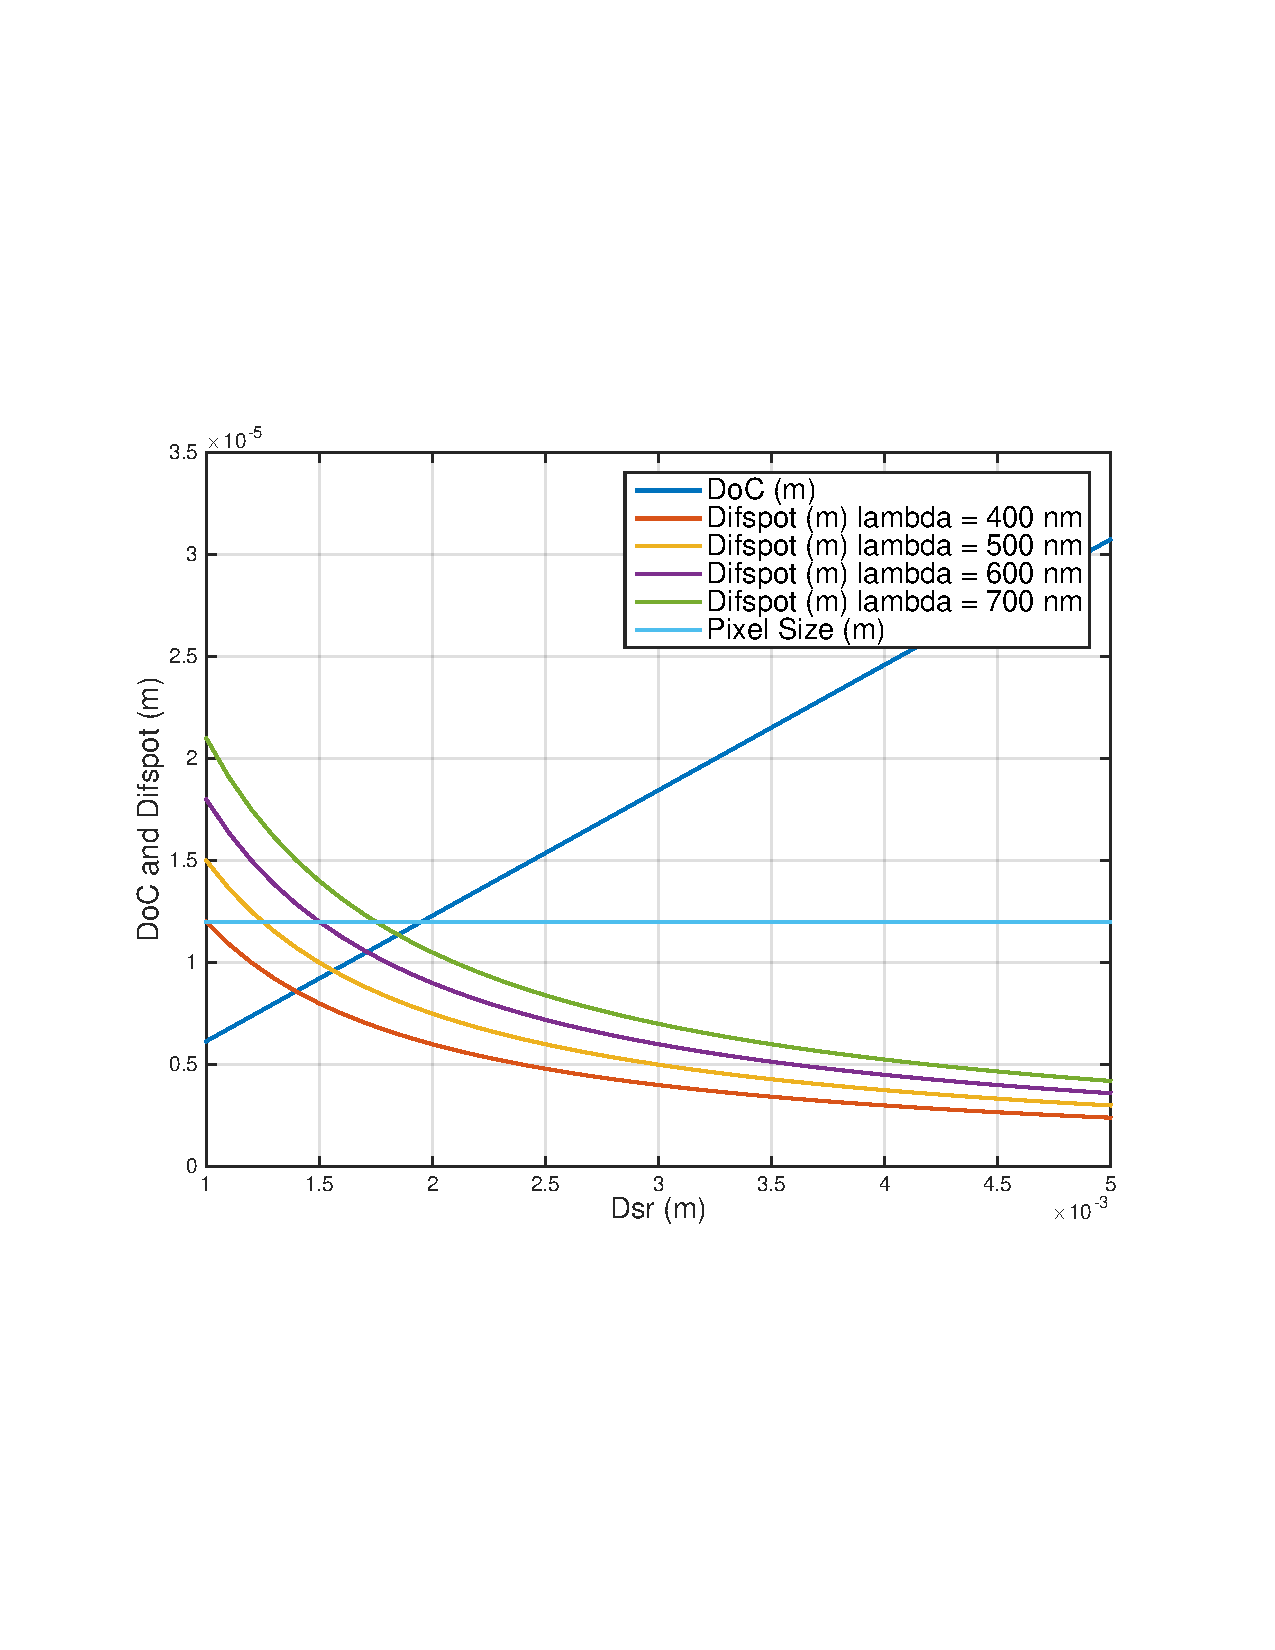
\includegraphics[trim=2cm 7cm 2cm 7cm, clip=true, totalheight=0.45\textheight, angle=0]{fig/DoCDifspot.pdf}
  \caption{Diameter of confusion and diffraction spots as a function of the diameter}
  \label{fig:DoCDifspot}
\end{figure}

Then, the depth of field can be deduced:
\begin{equation*}
DoF = \frac{2\frac{f}{Dsr}DoC(m+1)}{m^2 - (\frac{DoC}{Dsr})^2} = 1.33 \ m
\end{equation*}
That means that the roughness of the rock analysed cannot be more than $\frac{DoF}{2} =  66.5\ cm$ since we could not see the whole rock if not, and the 3D map will then be flawed.
First of all, the irradiance $F$ of the light from the sun falling at the top of the atmosphere of Mars can be calculated as following :
Conservation of energy :
\begin{equation}
\label{eq:conservation of energy}
4\pi R_\odot^2F_\odot=4\pi R^2F
\end{equation}
with 

$R_\odot=6,956.10^8\ m$ : solar radius

$F_\odot=6,45.10^7\ W.m^{-2}$ : energy flow of the surface of the sun

$R \in [2.06644,\ 2.49228].10^{11} \ m$ : distance Mars-Sun (Aphelion and Perihelion)

\begin{equation}
\label{eq:Irradiance Sun range}
F = F_\odot \left(\frac{R_\odot}{R}\right)^2 \in [502, 730]\ W/m^2
\end{equation}

In this report, we will consider that the rover is working on a specific date and we will chose the one when $R$ corresponds to the semi-major axis. In this case $R=2,27936.10^{11}\ km$ and
\begin{equation}
\label{eq:Irradiance Sun}
F = 589\ W/m^2
\end{equation}



Moreover, we can assume that a part of the irradiance is absorbed by the atmosphere. Knowing that the atmosphere of Earth absorbs and scatters to space around 30\% of the incident irradiance of the Sun\cite{yamamoto1962direct}, and knowing  that the atmosphere of Mars is thinner than the one of the Earth, we will postulate that 10\% of the incident irradiance is absorbed. Thus, using \ref{eq:Irradiance Sun} the actual irradiance $F_a$ of the light from the sun falling on the surface of Mars is

\begin{equation}
\label{eq:Actual Irradiance Sun}
F_a = \frac{90}{100}F = \frac{90*589}{100} = 530\ W/m^2
\end{equation}

However, this irradiance is the one of surface exposed perpendicular to the sun's beams. As Mars is a sphere, the projection need to be considered.
Knowing that the weather is better into the northern hemisphere of Mars\cite{wiki:weather} and the fact that a latitude between 30 an 70 degrees is favored for a landing\cite{latitude}, we will assume that the rover has a latitude of 50\textdegree. This latitude corresponds to an angle of 40\textdegree$\ $between the surface of Mars and the sun's beams. Moreover, suppose that the rover stop working when this angle is inferior to 10\textdegree. Thus, the irradiance $F_{50}$ at a latitude of 50\textdegree$\ $is

\begin{equation}
F_{50} = F_asin(angleBeams) \in [92, 341] \ W/m^2
\end{equation}

with $angleBeams = [10, 90-latitude] = [10, 40]$\textdegree.


Then, considering the trajectory of the Sun into the sky of Mars and knowing that the rock target is more or less vertical to the surface of Mars, the angle $\theta$ between the target's normal and the sun's beam is considered to be included in $[10, 50]$\textdegree. In addition, in the optimal case (when all the optimal conditions are provided to have the maximal radiance), the BRDF of the surface of the target is assumed to be 90\% Lambertian and 10\% Glossy while in the worst case the BRDF will be only Lambertian. In this way, the radiance of the target $R_T$ is

\begin{equation}
\label{eq:Radiance Target}
R_T = \left\{
	\begin{array}{ll}
		\frac{F_{50}\alpha}{\pi}\cos \theta & \mbox{ optimal case} \\
		F_{50}\alpha(\frac{9}{10\pi}\cos\theta + \frac{1}{10}) & \mbox{ worst case}
	\end{array}
\right.
\end{equation}

with 
\begin{align*}
	\alpha & \in [0.05, 0.45]\mbox{, the albedo of the target\ref{albedo}} \\
	\theta & \in [10, 50]\mbox{\textdegree, the angle between the target's normal and the sun's beam}
\end{align*}
Thus, 
\begin{equation}
R_T \in [92, 340] \ W/m^2
\end{equation}







\appendix
\chapter{LED Properties}
\label{LEDdatasheet}
\begin{figure}[h]
  %\centering
  \centerline{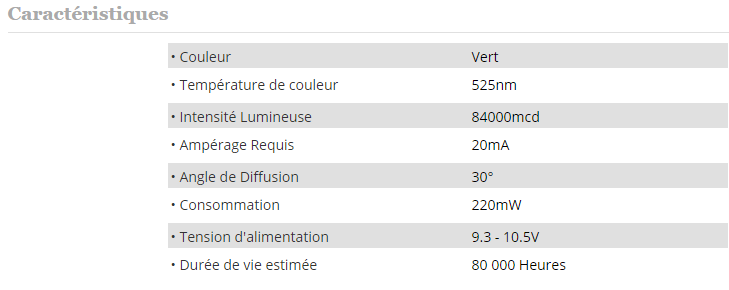
\includegraphics[scale=0.8]{fig/LedDataSheet.png}}
  \caption{LED Datasheet}
  \label{fig:LEDdatasheet}
\end{figure}

\chapter{CCD Properties}
\label{CCDdatasheet}
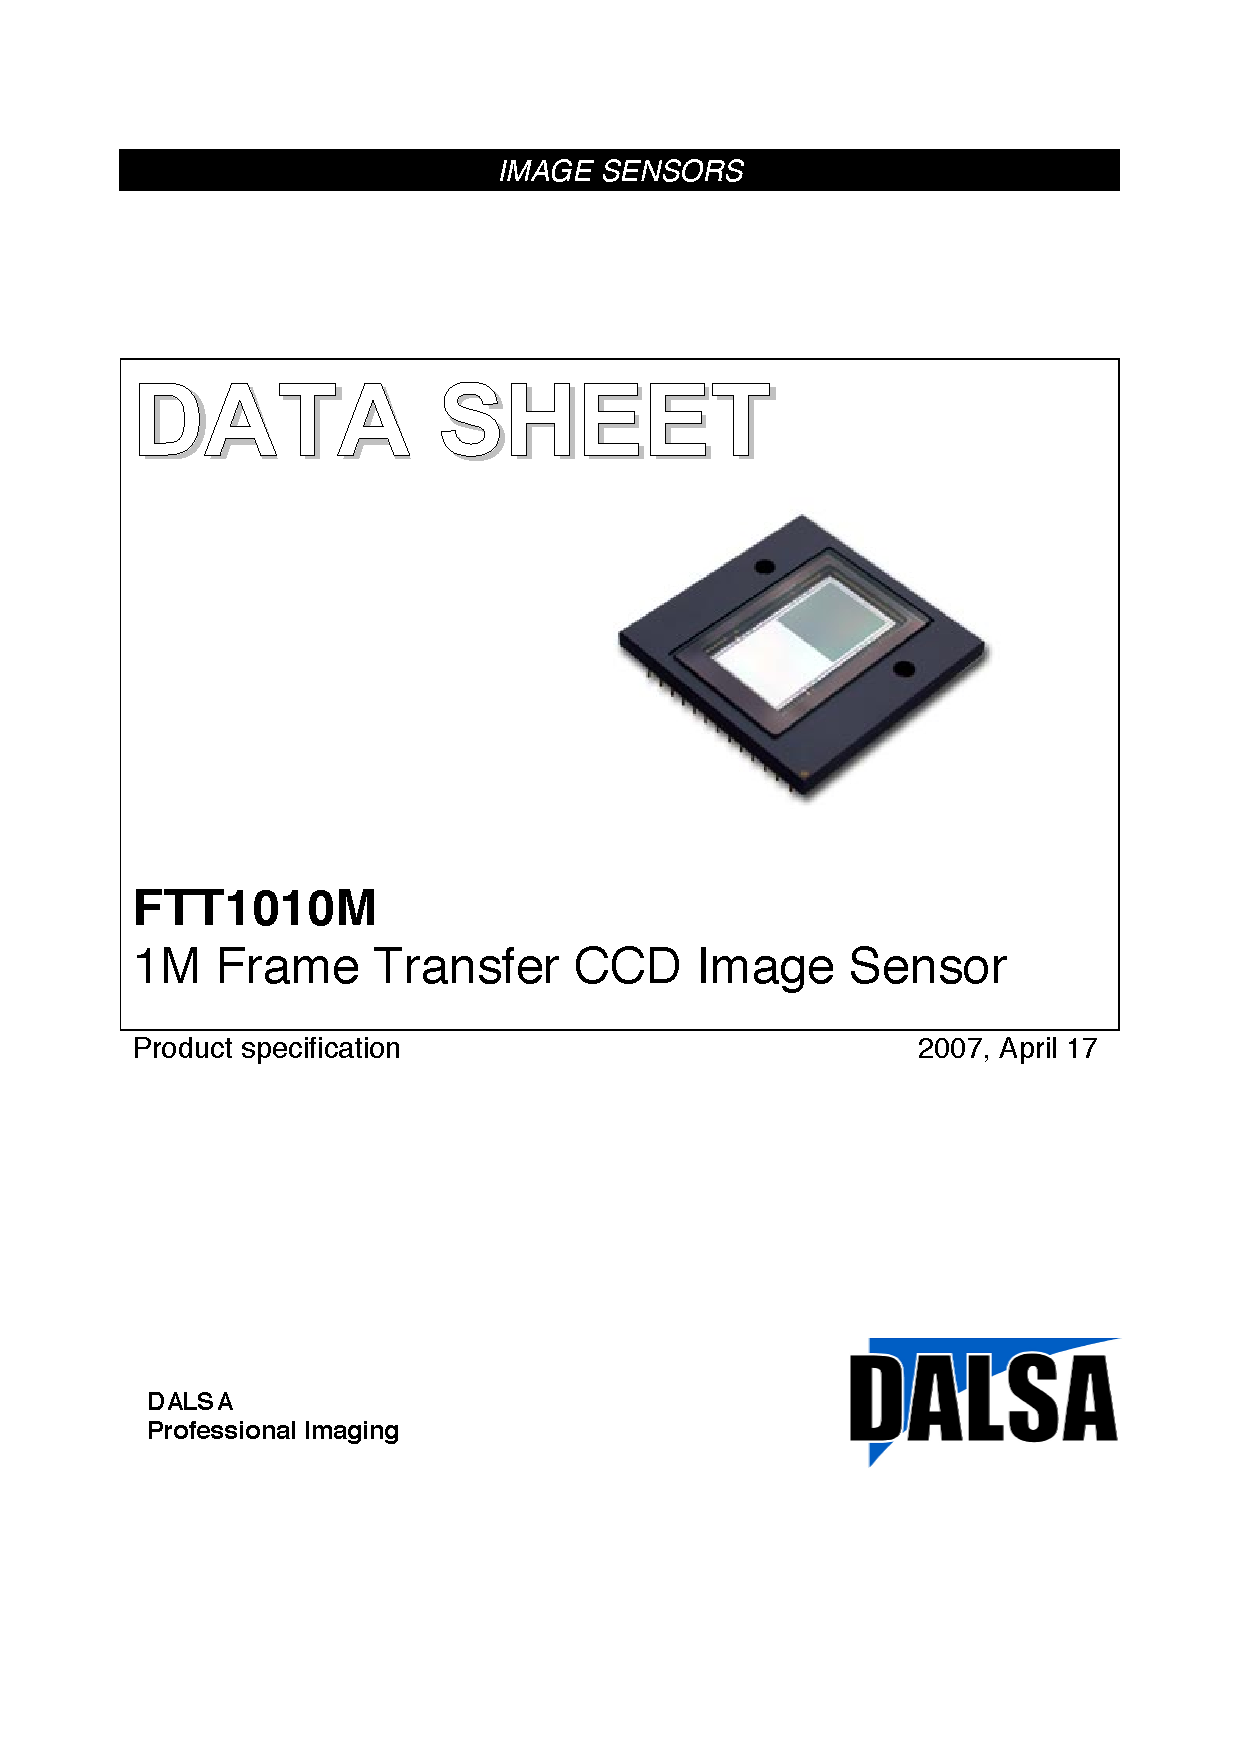
\includepdf[pages = {1-18}]{fig/CCDdatasheet.pdf}

%\end{appendices}

\bibliography{bibliographie}
\bibliographystyle{plain}

\end{document}
